% Setup - do not change
\documentclass[11pt]{article}
\usepackage[top=0.9in, left=0.9in, bottom=0.9in, right=0.9in]{geometry} 
\usepackage{parskip}

\usepackage{caption}
\usepackage{subcaption}
\usepackage[english]{babel}
\usepackage[utf8]{inputenc}
\usepackage{amsmath,amsthm,amssymb,graphicx,pdfpages,lipsum,hyperref}
\usepackage[none]{hyphenat}
\usepackage{csquotes}
\usepackage{float}
\usepackage[normalem]{ulem}
\useunder{\uline}{\ul}{}
\usepackage{booktabs}


\setlength\parindent{0pt}
%%%%%%%%%%%%%%%%%%%%%%%%%%%%%%%%%%%%%%%%%%%%%%%%%%%%%%%%%%%%%%%%%%%
% add other packages here if required

%% Bibliography are specified in this file. You can also choose inline bib style if you want to. But make sure your citation style is consistent (and proper)
% For more details on citation: https://library.unimelb.edu.au/recite
\usepackage[sorting = none]{biblatex}
\addbibresource{references.bib}

%%%%%%%%%%%%%%%%%%%%%%%%%%%%%%%%%%%%%%%%%%%%%%%%%%%%%%%%%%%%%%%%%%% the '%' symbol denotes comments

% Begin document creation
% DELETE THE \lipsum PLACEHOLDERS WHEN YOU BEGIN
\title{\textbf{Taxi fare forecasting using Gradient Boosted Trees} \\}
\author{
Noah Sebastian \\
Student ID: 911150 \\
%% Replace the link with your github repo
% 1. Remember to escape underscore (\_) in the link.
% 2. Remember to include the commit you want to submit in the link
\href{https://github.com/MAST30034-Applied-Data-Science/mast30034-project-1-911150/commit/b69920f80525f1fb42052ef7958d6927dcfa679b}{Github Repository (Remote Branch) [b69920f]}
}

\begin{document}
\maketitle

\section{Introduction}
On demand vehicle services play an essential role in providing convenient and affordable travel for individuals. 
Taking advantage of consumer demand for convenience and flexibility, technologically progressive companies such as Uber and Lyft have exploded onto the scene and now capture a significant proportion of the ride hail service, leaving the traditional taxi behind in the process. 

An aspect of the New York City (NYC) taxi service, and one that differs from the more modern on-demand-vehicles, is their inability to present end-to-end fare prices and inform individuals pre-travel about their future incurred costs. This is an area where for-hire-vehicles (FHV's) have a significant competitive advantage over the taxi industry.

As such, this report will assume the perspective of a research and development company working on behalf of the New York City Taxi \& Limousine Commission (NYCTLC) to provide insights and prospectus integration's for the current NYCTLC system and, more specifically, will attempt to offer a method for forecasting trip fare amounts for varying circumstances around New York City.

For this task, a Gradient-Boosted-Tree Regressor is suggested as such a model since it is capable of handling imperfect data sets, can generalize well and offers high flexibility. It is also currently one of the more mainstream algorithms adopted by the data science community. 
It will be contrast against a Random Forest Decision Tree Regressor, with the intention of exploring their differences, and effectiveness'.


% You can have \section{}, \subsection{}, and \subsubsection{}
\section{Dateset}

The NYC Taxi \& Limousine Commission record and report monthly statistics \cite{nyctlc}  on the trips undertaken by NYC's taxi’s (Yellow, Green), for-hire-vehicles and high-volume-for-hire-vehicles (Uber, Lyft, Juno, Via). 
This dataset provides rich information into the process’ that dictate taxi travel and fares.
The dataset contained a variety of features These were reduced for forecasting and analysis according to the case objective, as detailed in section !!.  

In addition to this, hourly historical NYC Meteorological Aerodrome Report (METAR) \cite{metar} data was also acquired and integrated into the model as it is hypothesized that its features could have a statistically relevant relationship with the predictor variable. \#XXXPUT THIS SOMEWHERE ELSE 
The features selected include temperature, relative humidity and dew point, as from these, most common weather types can be inferred.

\subsection{Range Selection}
As this report assumes the perspective of a ‘\# nyc taxi technological innovation guy making a pitch\#, it is necessary to provide a representation of what could be capable and achievable by the TLC using existing technologies, and limited resources.
As such, a subset of the Yellow Taxi dataset was selected. All trips that occurred during 2019, ($\approx 84.6$m records) were used for pre-processing, model training and analysis. Further, all trips recorded in 2021 ($\approx 30.9$m records) were used to validate and evaluate model performance. 

A more recent feature set would have been preferred for training, but due to concerns over the extreme effects COVID-19 \& Lock downs may have had over the taxi industry, they had to be ommitted.


\subsection{Feature Selection}
Due to the specific intentions of the report and subsequently the modelling, significant restrictions had to be imposed on the feature set. That is, any features that would not be available before a taxi ride commences, were removed. 
To comply with this, and still propose insightful findings, some realistic assumptions were made:
\begin{itemize}
    \item \textbf{Trip distance/duration} could be estimated by use of a modern GPS system e.g. (Google Maps, TomTom) and as such can be retained as a feature.
    \item \textbf{Congestion and their consequent surcharges} are considered to be similarly estimable.
    \item \textbf{Instantaneous weather data} is available and accessible.
    \item \textbf{Location specific variables} such as Ratecode etc. could be generated from destination information.
\end{itemize}

This gave the following feature set:

\begin{table}[H]
\centering
\begin{tabular}{cccl}
\multicolumn{2}{c}{\textbf{Retained Features:}} & \multicolumn{2}{c}{\textbf{Weather data Features:}} \\
Date \& Time     & Ratecode ID’s        & \multicolumn{2}{c}{Temperature}       \\
Passenger Counts & Location ID’s        & \multicolumn{2}{c}{Dew Point}         \\
Trip Distance    & Payment Types        & \multicolumn{2}{c}{Relative Humidity} \\
Fare amounts     & Congestion surcharge & \multicolumn{2}{l}{}                 
\end{tabular}
\end{table}


In order to increase information from the data, the following features were engineered using the original set:
\begin{itemize}
    \item Hour of day (PU/DO)
    \item Day of week (PU/DO)
    \item Day of month (PU/DO)
    \item Month of year
    \item Trip Time (minutes)
    \item Trip speed (mph)
    \item Fare per minute
\end{itemize}



\subsection{Collation}
Aggregation was required when joining the weather and taxi data sets. The METAR data came with sub-hourly samples. Since the lowest time unit that had been engineered was hourly, the weather data was mean aggregated across these intervals before merging. 

Since the weather data was relatively comprehensive and due to the abundance of trip records, any inconsistencies in matches resulted in the records being dropped from analysis.


\subsection{Outlier Analysis}
Although the data sets were generally well formed, the taxi dataset contained a significant amount of outliers and discrepancies that would hinder the performance of the model if left unaddressed. 

In accordance with sound data literacy principles, the taxi dataset underwent significant processing and outlier handling:

\textbf{Trips with negative and over 312 (miles)} were removed. Any trips longer than 312 (miles) were considered to be beyond the scope of analysis. \#more how did you come up with this number?

\textbf{Trips with Location ID’s outside the range 1-263 were removed.} This is in line with the specifications provided in the data dictionary \cite{nyctlc_dd}.

\textbf{Trips with Fare Amounts greater than \$500.} These trips were investigated and concluded to be predominantly noise/input error.

\textbf{Trips with passenger counts greater than six people.} According to the NYCTLC guidelines \cite{nyctlc_pass} regarding 'Overloading Vehicles'. A driver must not permit more than five passengers, but is allowed an additional passenger riding on the lap of their guardian, giving at most 6.

\textbf{Trips with negative tip amounts} were removed. These were consistent with similar negative values found in other features. No pattern was identifiable to these outliers and as such they had to be dropped.

\textbf{Trips with Vendor ID’s outside the specified range.} Guidelines state that only vendor codes 1 and 2 are registered as valid TPEP providers\cite{nyctlc_dd}.

\textbf{Trips filtered to only contain credit card or cash Payment Types.}

\textbf{Trips with Ratecode ID’s outside valid bounds were removed.} Specifications report Ratecodes 1 to 6 as the only valid rate codes being in effect subject to the end of the trip.

\textbf{Trips with average speed (mph) greater than 65 mph and less than 1 mph were removed.} NYC state guidelines \cite{nyctlc_pass} report the inner-city speed limit as 50 mph, and the interstate speed limit as 65 mph and it is assumed that taxi drivers mostly adhere to these restrictions. 

\textbf{Trips with travel speeds under 1 mph were considered noise/outliers.}

\textbf{Trips with Standard Ratecodes and Fare amounts under \$2.50 were removed.} In line with NYCTLC guidelines trips with standard ratecodes have an initial fee of \$2.50, so any fare's fitting this description, under this price, were removed.

After processing the data sets contained $\approx 71.7$m and $\approx 26.7$m records for 2019 and 2021, respectively.

\subsection{Imputation}
After strict outlier removal process, there were no longer any missing values and no imputation was required.

\section{Preliminary Analysis}
This section will serve to identify relationships between the feature set and the variable of interest (Fare Amount) and also the available investigate categorical descriptors.

In order to feasibly provide visualization, sub-sampling without replacement was performed to down-sample the set to a more manageable size. The sampling was performed at random from the entire collated data set, with the intention of capturing enough distributional information to present graphically.

XXXX\#
The primary question this section intends to answer is: \textbf{what constitutes a taxi's fare amount?} and of the features we have restricted ourselves too: \textbf{how can we forecast this feature}? 

To help aid the direction of analysis, a correlation matrix was plot for the relevant features (Figure \ref{fig:corrmatix}).

\begin{figure}[H]
    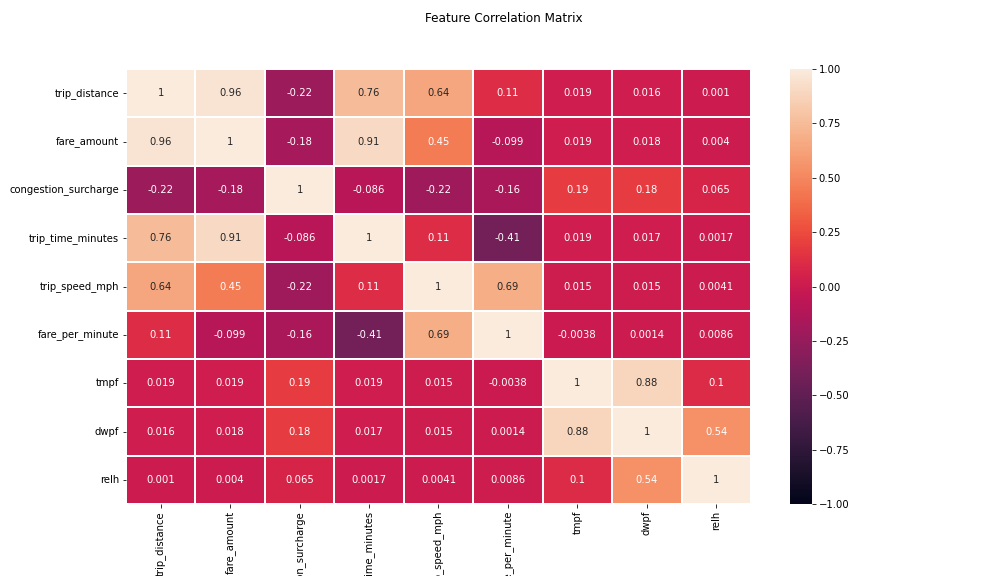
\includegraphics[width=1\textwidth]{corr_matrix.png}
    \centering
    \caption{Correlation matrix of the feature set}
    \label{fig:corrmatix}
\end{figure}


\subsection{Trip Duration}
It was assumed that trip duration would have significant correlation with cost of the trip. 
This is confirmed when observing the correlation matrix. Can see that the trip duration and fare amount features are highly correlated (0.96).
This is unsurprising due to distance travelled being a main constituent in how taxi fares are formulated; Specifically, the charge is increased by 50 cents for every 0.2 miles when travelling above 12 mph\cite{nycfarepage}.

\subsection{Trip Time}
Again, it would be assumed that trip time and fare amount should be highly correlated; and they are (0.91). Trip time is also a constituent in fare calculation, but is only used when travelling below 12 mph. More specifically, for every 60 seconds that is spent under 12 mph, an additional 50 cents is charged\cite{nycfarepage}.

This is interesting, as one would imagine that a significant amount of trips would average speeds much faster than this, and therefore trip time should not be such a strong predictor.

\#\#\# XXX
An explanation for this, is trip times extremely high positive correlation with distance (0.96); and we know that trip duration is an excellent predictor of fare amount, hence via proxy correlation, as is trip time.

\subsection{Congestion Surcharge}
Congestion surcharge had a reasonably significant negative correlation with fare amount (-0.18). This garnered uni/bivariate investigation of the feature (Figure \ref{fig:congeston}). It can be seen that there are two prominent bands  in the distribution of the feature. This banding was found to be explained by the way congestion surcharge is calculated. Fare guidelines state that any trips that at any point pass south of 96th Street, Manhattan, incur a \$2.50 charge\cite{nycfarepage}.


\begin{figure}[h]
     \centering
     \begin{subfigure}[b]{0.45\textwidth}
         \centering
         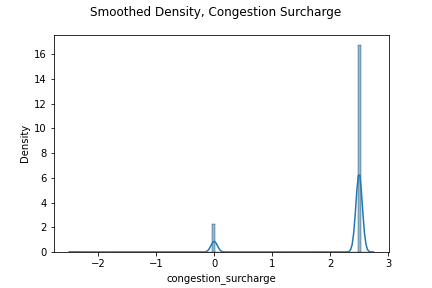
\includegraphics[width=\textwidth]{congestion_surcharge_density.png}
         \caption{Congestion Surcharge Distribution}
         \label{fig:y equals x}
     \end{subfigure}
     \hfill
     \begin{subfigure}[b]{0.45\textwidth}
         \centering
         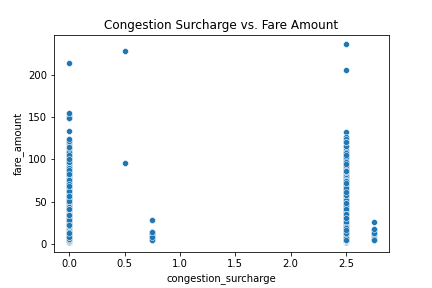
\includegraphics[width=\textwidth]{con_vs_fare.png}
         \caption{Congestion Surcharge vs. Fare Amount}
         \label{fig:three sin x}
     \end{subfigure}
        \caption{Congestion surcharge distribution and relationship with Fare amount}
        \label{fig:congeston}
\end{figure}


\subsection{Distributional Analysis}
Trip distance and duration were selected for a closer look as they showed compelling correlations with fare amount.

The pair plot (Figure \ref{pair}) shows their relationships. It can be noticed in (Figure \ref{fig:pairplots})(a) that their distributions all present long right-tails, and are positively skewed.

It was hypothesised that a natural log transformation could present a more normal depiction of these features, and observing (Figure \ref{fig:pairplots})(b) it can be seen that the extreme tail behaviour is much more Gaussian.

Further, the pairs show strong linear relations, suggesting they will be effective in forecasting their counterparts.

\begin{figure}[H]
     \centering
     \begin{subfigure}[b]{0.45\textwidth}
         \centering
         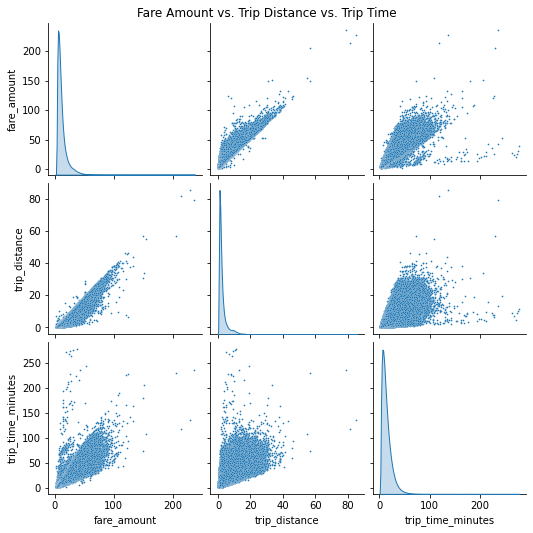
\includegraphics[width=\textwidth]{features_pairplot.png}
         \caption{No transformations}
         \label{fig:y equals x}
     \end{subfigure}
     \hfill
     \begin{subfigure}[b]{0.45\textwidth}
         \centering
         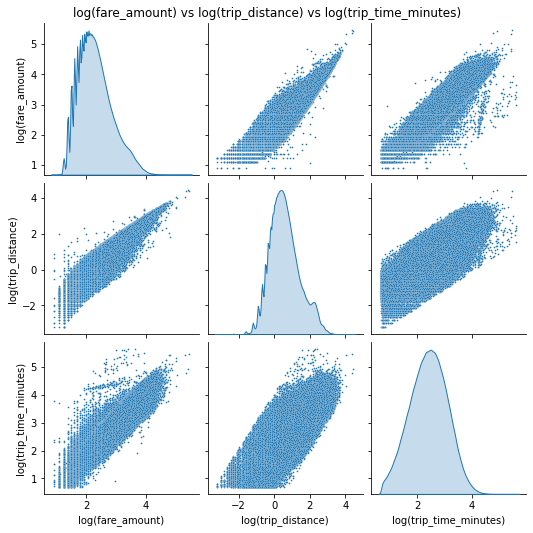
\includegraphics[width=\textwidth]{log_features_pairplot.png}
         \caption{Natural Log transformation applied}
         \label{fig:three sin x}
     \end{subfigure}
        \caption{Pairwise plot's of the Fare Amounts, Trip Times, Trip Durations and their respective Log transformations.}
        \label{fig:pairplots}
\end{figure}


% Please add the following required packages to your document preamble:
% \usepackage{graphicx}
\begin{table}[h]
\resizebox{\columnwidth}{!}{%
\begin{tabular}{l|c|c|c|c|c|}
\cline{2-6}
 &
  \multicolumn{1}{l|}{Trip Distance} &
  \multicolumn{1}{l|}{Tip Amount} &
  \multicolumn{1}{l|}{Passenger Count} &
  \multicolumn{1}{l|}{Fare Amount} &
  \multicolumn{1}{l|}{Congestion Surcharge} \\ \hline
\multicolumn{1}{|l|}{Mean}    & 2.5890   & 2.0484   & 1.5950   & 11.9264  & 2.2457   \\ \cline{1-1}
\multicolumn{1}{|l|}{St. dev} & 2.8275   & 2.1992   & 1.2037   & 8.3485   & 0.7611   \\ \cline{1-1}
\multicolumn{1}{|l|}{Max}     & 0.04     & 0.0      & 1.0      & 2.5      & 0.0      \\ \cline{1-1}
\multicolumn{1}{|l|}{Min}     & 149.5    & 500.0    & 6.0      & 394.5    & 2.75     \\ \hline
\end{tabular}%
}
\caption{Post processing descriptive statistics of the features}
\label{tab:descriptive-statistics}
\end{table}



\section{Gradient Boosted Tree (GBT) \& Random Forest (DT) Regression}
In Gradient Boosting Decision Trees multiple weak form models (Decision Trees) are combined via ensemble methods to produce a singular greater model. The individual decision trees are connected in series, where each new tree's goal is to minimise the error of its predecessor. 

The sequential nature of this 'boosting' process means that the algorithms are typically slower to learn, but can produce higher accuracies. This will be analysed when comparing the bagging methods of Random Forests with the GBT methods.

Due to decision trees being flexible with their inputs, no encoding or scaling was performed, but the features were vectorised in order to implement the machine learning libraries of PySpark\cite{pyspk}.

The models were trained on the 2019 data set. This would not normally be the case, but to be in line with subject specification, additional data was required for testing the models.

Predictions were then made on the set and evaluated. The metrics used to evaluate the models were: Root Mean Square Error (RMSE), Mean Absolute Error (MAE), Mean Squared Error (MSE), Explained Variance and Coefficient of Determination ($R^2$).

\begin{table}[H]
\centering
\begin{tabular}{l|c|c|c|c|c|}
\cline{2-6}
                          & \multicolumn{1}{l|}{RMSE} & \multicolumn{1}{l|}{MAE} & \multicolumn{1}{l|}{MSE} & \multicolumn{1}{l|}{Exp.Variance} & \multicolumn{1}{l|}{R2} \\ \hline
\multicolumn{1}{|l|}{GBT} & 1.7055                    & 0.7775                   & 2.9086                   & 63.7937                           & 0.9563                  \\ \hline
\multicolumn{1}{|l|}{RF}  & 1.9801                    & 0.9406                   & 3.9207                   & 52.6606                           & 0.9411                  \\ \hline
\end{tabular}
\caption{Prediction Results for the Gradient Boosted Tree model and the Random Forest model,}
\label{tab:pred_results}
\end{table}

The results (Table \ref{tab:pred_results}) followed expectations regarding GBT and RF trees. The Gradient Boosted Tree outperformed the Random Forest across the metrics, although it cannot be said that the Random Forest Model performed poorly. In fact, both models performed remarkably well; that is, they were able to on average predict true fare amounts to within (0.7775) and (0.9406) (USD) respectively over the test set. The feature importance's were then investigated to understand which attributes are contributing to the successes of the models (Table \ref{tab:feature_importances}).

\begin{table}[H]
\resizebox{\columnwidth}{!}{%
\begin{tabular}{llllll}
 & \multicolumn{2}{c}{\textbf{Random Forest}}          &  & \multicolumn{2}{c}{\textbf{Gradient Boosted}}       \\ \cline{2-3} \cline{5-6} 
 & \multicolumn{1}{l|}{Feature Name} & Feature Importance (\%) &  & \multicolumn{1}{l|}{Feature Name} & Feature Importance (\%) \\ \cline{2-3} \cline{5-6} 
 & \multicolumn{1}{l|}{Trip distance (miles)} & 0.5394 &  & \multicolumn{1}{l|}{Trip distance (miles)} & 0.7513 \\
 & \multicolumn{1}{l|}{Trip time (minutes)}   & 0.3640 &  & \multicolumn{1}{l|}{Trip time (minutes)}   & 0.2260 \\
 & \multicolumn{1}{l|}{Trip speed (mph)}      & 0.0610 &  & \multicolumn{1}{l|}{Trip speed (mph)}      & 0.0213 \\
 & \multicolumn{1}{l|}{Pick-up LocationID}    & 0.0252 &  & \multicolumn{1}{l|}{Congestion Surcharge}  & 0.0009
\end{tabular}%
}
\caption{Top 4 highest scoring features (importance) for the Gradient Boosted and Random Forest Models.}
\label{tab:feature_importances}
\end{table}
Both models used similar features, the only difference being RF favoring Pick-up Location ID's over GBT's Congestion Surcharge as it's 4th highest ranking predictor.
What is more interesting is the distribution of importances'. The GBT model put heavier emphasis on Trip Distance (0.7513\%) against the RF model's (0.5394\%) importance. The correlation between trip distance and fare amount, combined with GBT's higher weighting could help to explain its out performance of RF. 


\subsection{Prediction Error Analysis}

In order to understand the errors in prediction and the model, it's predictions were visualised against their true values (Figure 5).

\begin{figure}[H]
     \centering
     \begin{subfigure}[b]{0.45\textwidth}
         \centering
         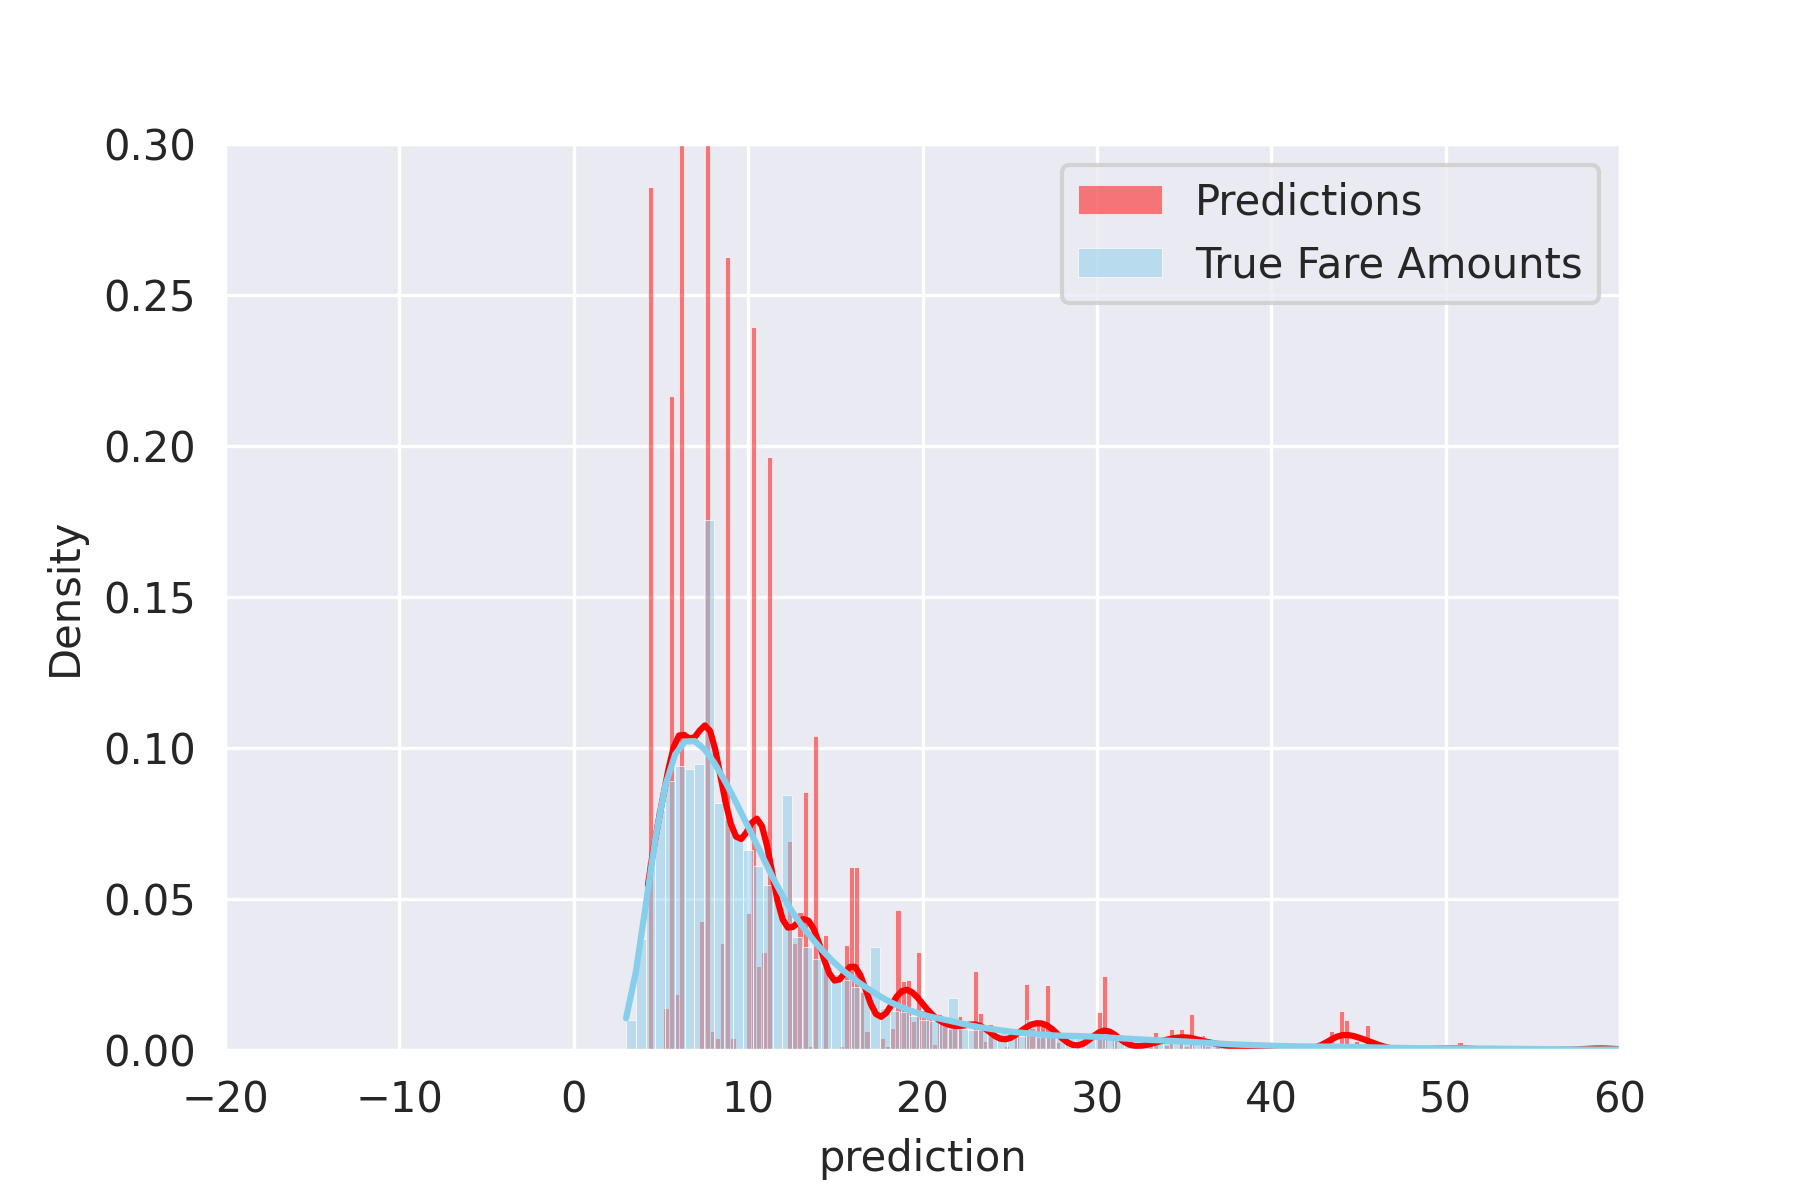
\includegraphics[width=\textwidth]{preds_vs_true.png}
         \caption{insert caption}
         \label{fig:y equals x}
     \end{subfigure}
     \hfill
     \begin{subfigure}[b]{0.45\textwidth}
         \centering
         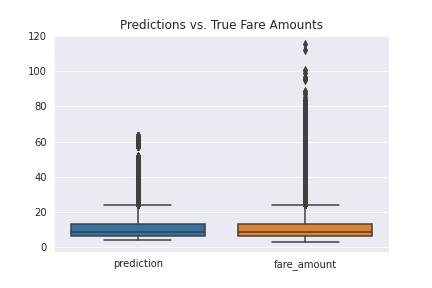
\includegraphics[width=\textwidth]{preds_vs_fare_boxplot.png}
         \caption{Predictions vs. True Fare Amount's Boxplot}
         \label{fig:three sin x}
     \end{subfigure}
        \caption{(Left) Histogram of Gradient Boosted Tree model's predictions and the true Fare Amounts for 2021 and respective box plots (Right)}
        \label{fig:three graphs}
\end{figure}

When visualising the GBT predictions versus the true fare amounts, it is worth noting the differences in concavity of the distributions. Unlike the true fare value distribution, the predictions do not follow a smooth slope, and instead display significant fluctuations, above and below, over and under estimating around the true values.

(Figure 4)(b) gives further insight to the limitations of the model. The whiskers of the box plots show that their is a deficiency in predicting large fare amounts. That is, at the tails of the data the model underestimates the true price. It is suggested that this could be addressed by collecting more data about these regions in turn allowing the model to make better informed predictions at the extremes. Further, transformations could be applied to the model inputs to regularize their behaviour.

\section{Discussion}

To reiterate, the aim of this report is to propose a method for forecasting taxi fare amounts in order to help the NYC Yellow Taxi overcome a significant disadvantage it has against HVFHV's. Considering the predictive power the models were able to achieve, and their general simplicity, this should be encouraging for NYCTLC or any offline for-hire-vehicle-service to pursue implementing or investigating this technology.

If the NYCTLC were able to incorporate this technology and perhaps extend into the digital booking fields, they could potentially create a new style of taxi driver. One who harmoniously moves between 'on-the-fly' pickup's and digitally requested rides. 

If this field of interest was to be extended, it is highly recommended to broaden the range of data. Space constraints limited the abilities for significant processing and training. Further outlier analysis, noise reduction and aggregation would be necessary, especially regarding older data sets.

Further improvements would have to be made in understanding the data sets distribution. Perhaps a GBT model, although generally applicable, would be outperformed by a model that more accurately fits the distribution and as a consequence can correctly approximate the tail behaviour. The tail behaviour is a significant pitfall in the models predictive capabilities.

Also, the GBT and RF Models would both benefit from hyper-parameter tuning. Due to the complexity of the data set, the computational costs of performing a Grid Search type operation could not be completed, but it would no doubt help to consolidate or improve results.

\section{Conclusion}
This report aimed to offer an insight into the feasibility of implementing an estimative service for fare amounts that could be appreciated by customers. Using NYCTLC trove of data regarding the trips by Yellow Taxi's, an in-depth analysis and learning process was able to showcase the power of modern decision tree algorithms and where they may under perform.


\clearpage

% BEGIN REFERENCES SECTION
\printbibliography

\end{document}


% the [h] ensures your figure is inline at the location and not displayed on some other page
\begin{figure}[h]
    % change the scale multiplier to make the figures smaller or larger
    \includegraphics[width=0.35\textwidth]{example-image-a}
    % this ensures your figures are centered where possible
    \centering
    \caption{Some caption} % refer to this image as (Figure 1)
\end{figure}




The features retained from the set were:
\begin{itemize}
    \item Date \& Time
    \item Passenger Counts
    \item Trip Distance
    \item Ratecode ID's
    \item Drop-off (DO) and Pick-Up (PU) Location ID's
    \item Payment Types
    \item Fare amounts
    \item Congestion surcharge
\end{itemize}

From the weather data:
\begin{itemize}
    \item Temperature
    \item Dew Point
    \item Relative Humidity
\end{itemize}


Else wise, if the data had been included, the set may have been (a) unmanageable with limited resources and time constraints and (b) produced forecasts that were less encompassing of ‘normal’ taxi behavior and as a result could fail to generalize to the LESS PANDEMICY \#totalitarian case.


